\section{Transmissão de Calor}

O objetivo do grupo de transmissão de calor, é auto explicativo. Determinar as temperaturas e influências térmicas existentes no sistema, prioritariamente no que tange à esfera da câmara de combustão e suas derivadas. Assim como analisar os riscos, determinar diretrizes à outros grupos e custos de materiais.

\subsection{Metodologia de trabalho}

Seguindo o seu objetivo, primeiro foram determinados o que seria de importância ao desenvolvimento do projeto como um todo, posteriormente o grupo de subdividiu em unidades individuais de forma que mais pesquisa pudesse ser realizada em menos tempo. Posteriormente foi subdividido novamente em tais equipes, conceito e documentação, simulações, tubulações e modelos matemáticos e físicos aplicáveis.

A determinação precisa do fluxo de calor é uma importante tarefa tanto para o projeto quanto para o cálculo do desempenho de motores foguete. No presente ponto de controle 2, o fluxo de calor na câmara de combustão de motores-foguete com geometria cilíndrica será calculado utilizando-se das equações newtonianas de temperatura e posteriormente será simulado por meio do programa ANSYS versão R18.1 e R18.2 Academic.

\subsection{Introdução}

Utilizando os conhecimentos anteriormente previstos foram determinados às equações que seriam utilizadas, após as pesquisas. Definimos então a equação da taxa de fluxo de calor, A equação de propagação de calor em cilindros no sentido radial.\\
$$ P_{cond} = \frac{\Delta Q}{\Delta t} = \frac{K.A.\Delta T}{L}$$
$$ Q_{cond} = k_{t}.4.\pi.r_{0}.r_{i}.\frac{T_{S0}-T_{Si}}{r_{0}-r_{i}}$$

\subsection{Analise teórica}
\subsubsection{Análise da câmara de combustão - Temperatura de parede}

A análise da câmara de combustão está relacionada à temperatura de parede, afinal o sistema de arrefecimento apenas está ligado a ela através do adaptador. 

De acordo com os dados disponíveis e com o conhecimento de que a câmara de combustão utilizada pela universidade é de tamanho laboratorial, muita bibliografia é existente nesse contexto, assim a base e logo conclusão da análise da temperatura de parede se deu com os seguintes gráficos abaixo. Na qual a temperatura sensível ao termopar é de $800^{\circ}C$ mas pela alta temperatura seu erro pode se estender em 20\%, o que é comprovado pela bibliografia que revela que a temperatura na câmara disposta às mesmas condições.

\begin{figure}[!htb]                                                               
   \centering                                                                      
   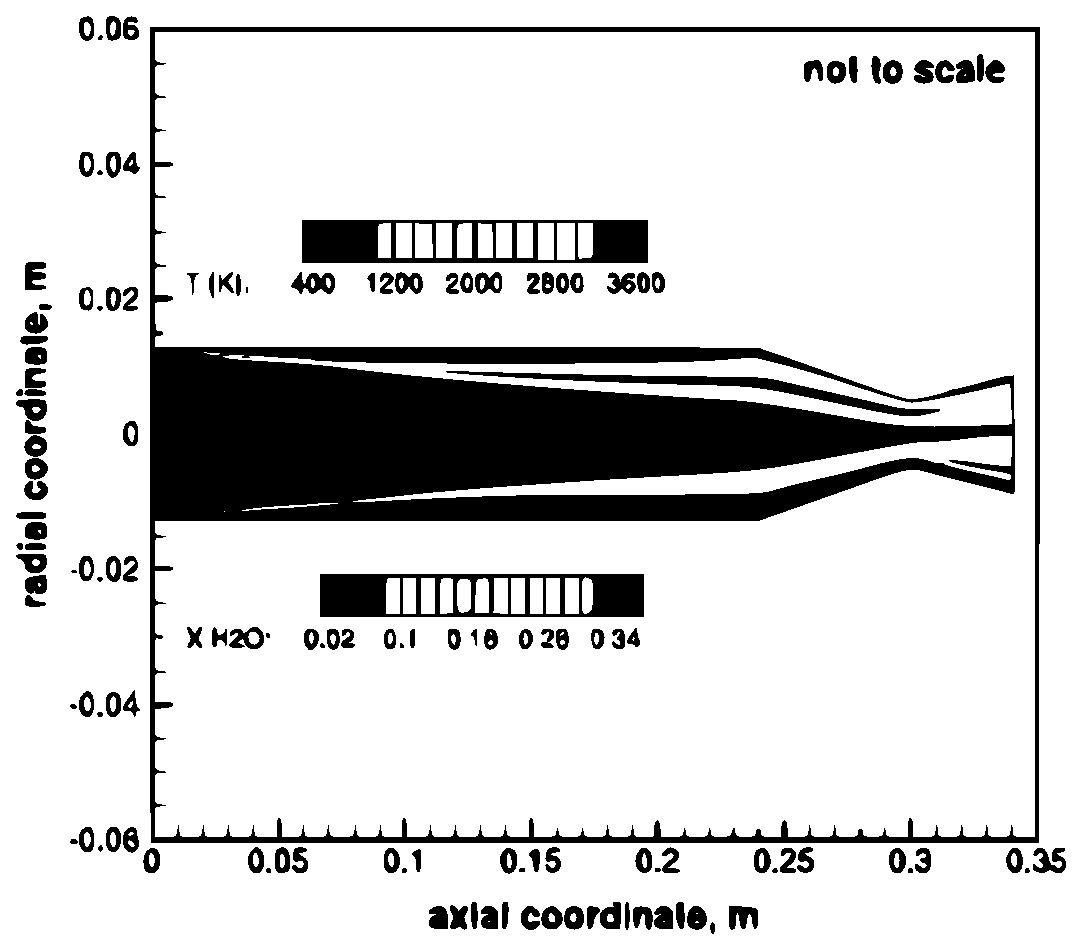
\includegraphics[keepaspectratio=true]{figuras/Camara1.eps}
   \caption{Esquemático geral do projeto de estrutura}                        
\end{figure}

\subsubsection{Análise do adaptador}
O adaptador é o fator determinante e o único conector da câmara ao sensor de forma que sua temperatura na ponta é adotada como a temperatura do sensor uma vez que são de materiais semelhantes, isto é aço inox, no caso do adaptador 304L.

\begin{figure}[!htb]                                                               
   \centering                                                                      
   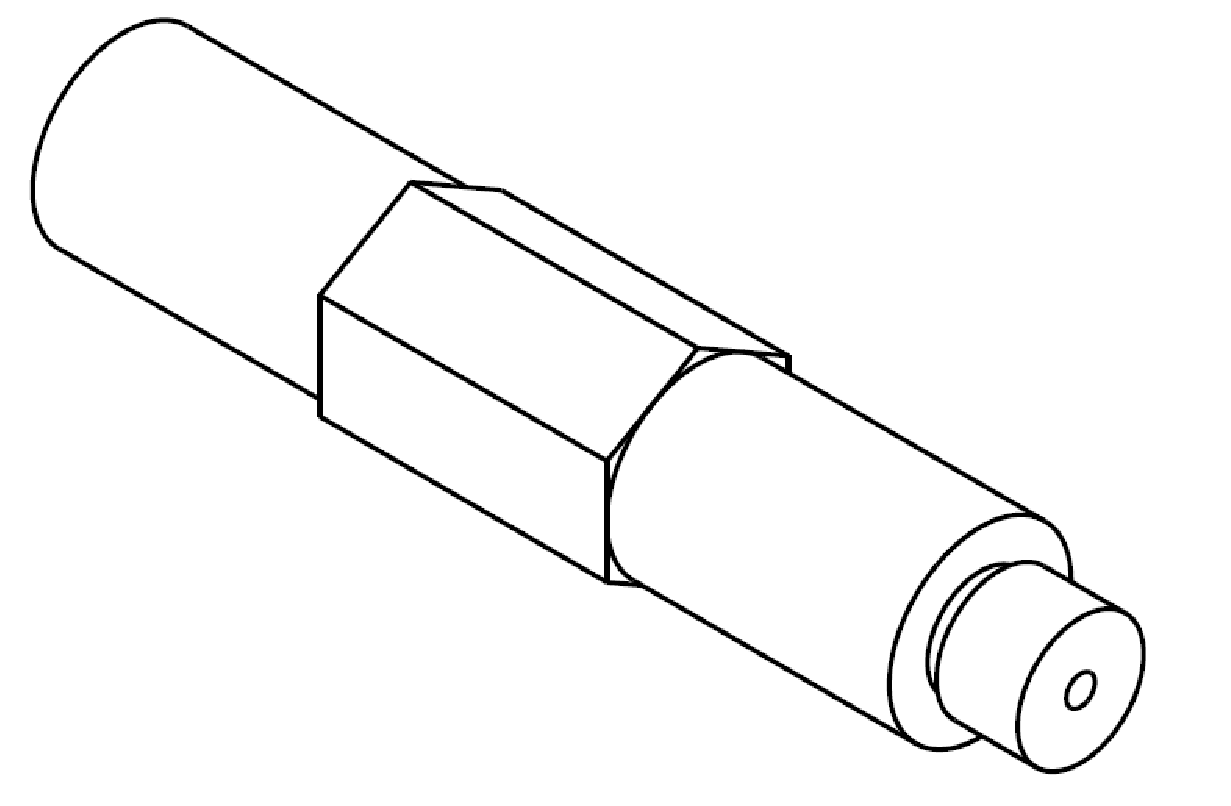
\includegraphics[keepaspectratio=true]{figuras/Parte1.eps}
   \caption{Esquemático geral do projeto de estrutura}                        
\end{figure}

Assim utilizando das suas propriedades foi então feita uma simulação para determinar sua temperatura de ponta, por admiti-lo como um cilindro perfeito. De diâmetro de 19mm e com comprimento de 100mm. Assim como às propriedades dele em temperatura de $1000^{\circ}C$ mais próximas encontradas na bibliografia são elas: Condutividade térmica - 21.4 W/K.m, Gradiente de condução - 25 no sentido da seção, temperatura ambiente de $30^{\circ}C$. Gerando o seguinte gráfico ANSYS.

\begin{figure}[!htb]                                                               
   \centering                                                                      
   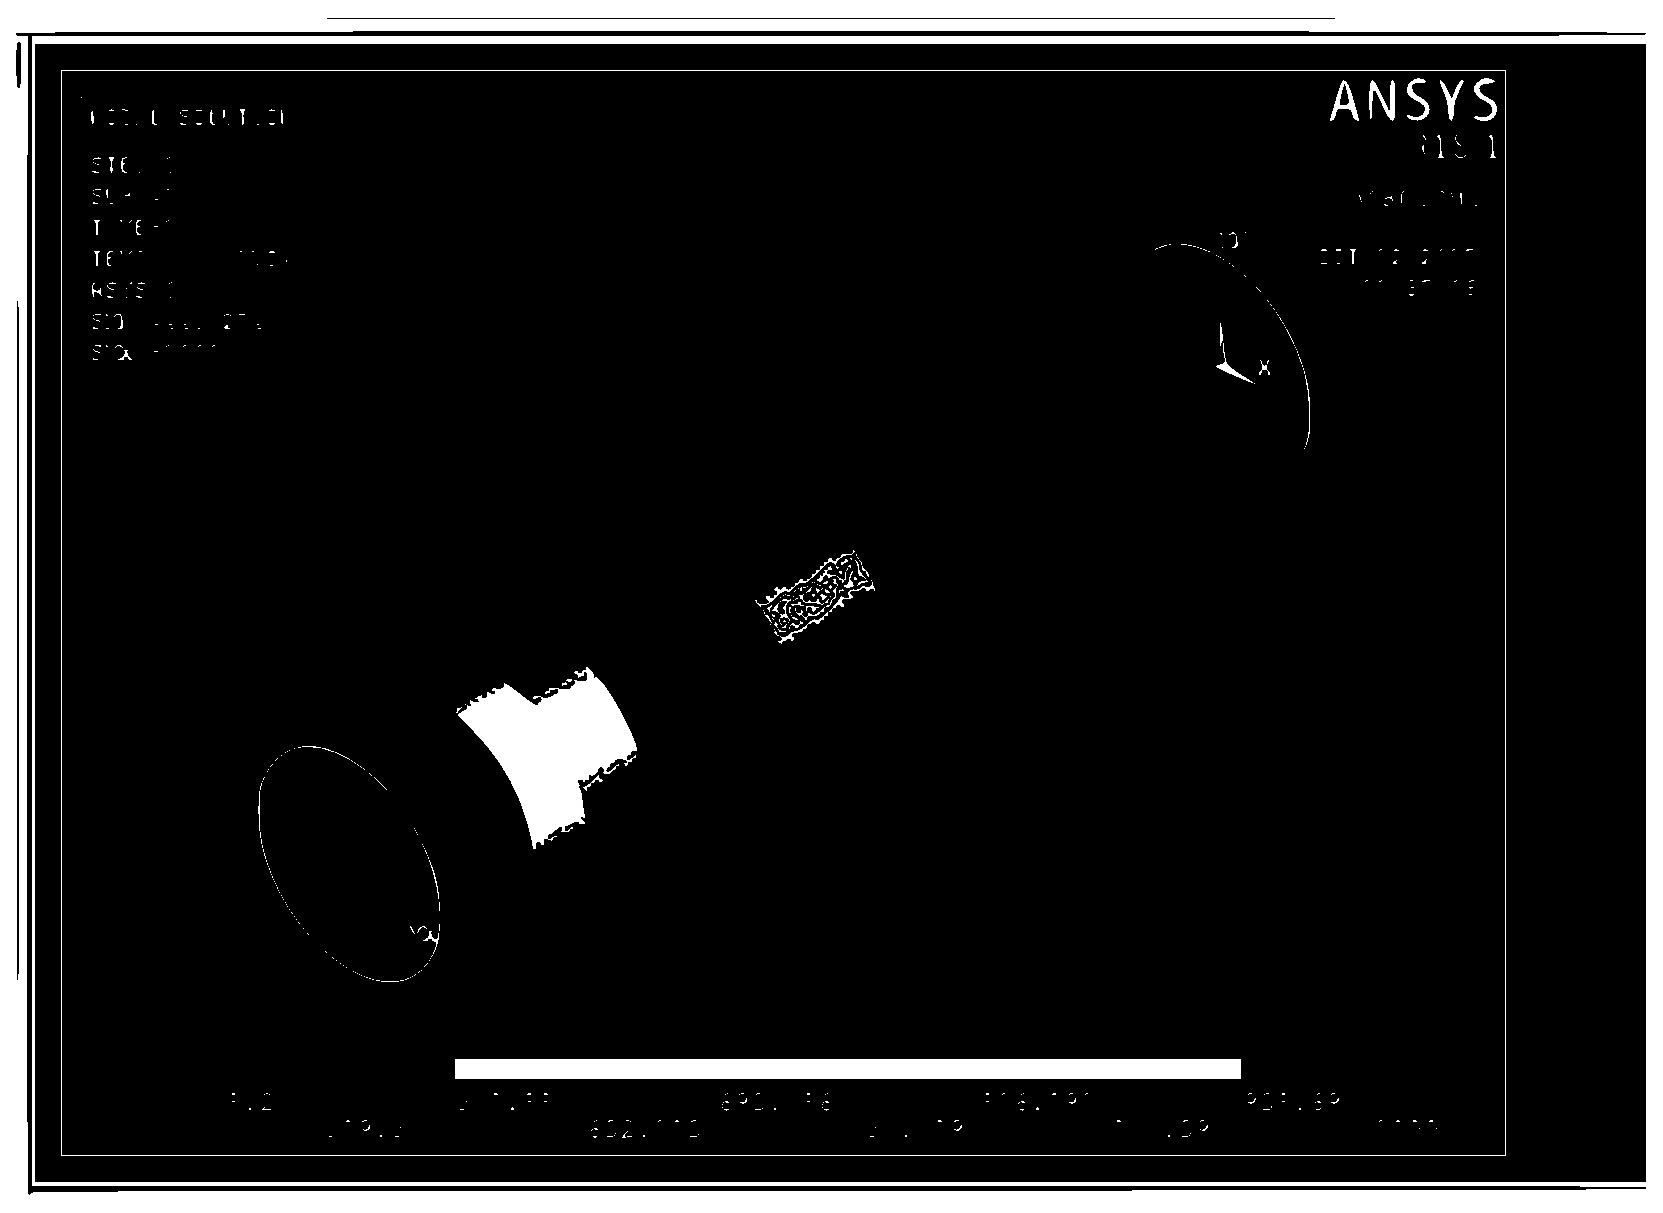
\includegraphics[width=15cm, keepaspectratio=true]{figuras/Resultado1.eps}
   \caption{Esquemático geral do projeto de estrutura}                        
\end{figure}

\begin{figure}[!htb]                                                               
   \centering                                                                      
   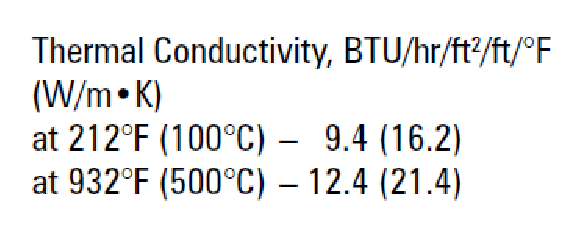
\includegraphics[width=15cm, keepaspectratio=true]{figuras/Teste14.eps}
   \caption{Esquemático geral do projeto de estrutura}                        
\end{figure}

\subsubsection{Análise de temperatura no sensor}
Como o sensor é feito majoritariamente de aço e sua massa é pequena demais, foi adotada sua temperatura como a da ponta do adaptador, dessa forma podemos assim cortar tempo em fazer contas extremamente pouco impactante no resultado final de forma que sua aplicação é apenas uma burocracia, visto que a utilização de fatores de segurança é o suficiente para a sua determinação com segurança.

\subsubsection{Análise da temperatura da água}
Após ser determinado que o líquido de arrefecimento é água, sua temperatura é facilmente determinada pela seguinte equação que resulta em $56.4^{\circ}C$.

\begin{figure}[!htb]                                                               
   \centering                                                                      
   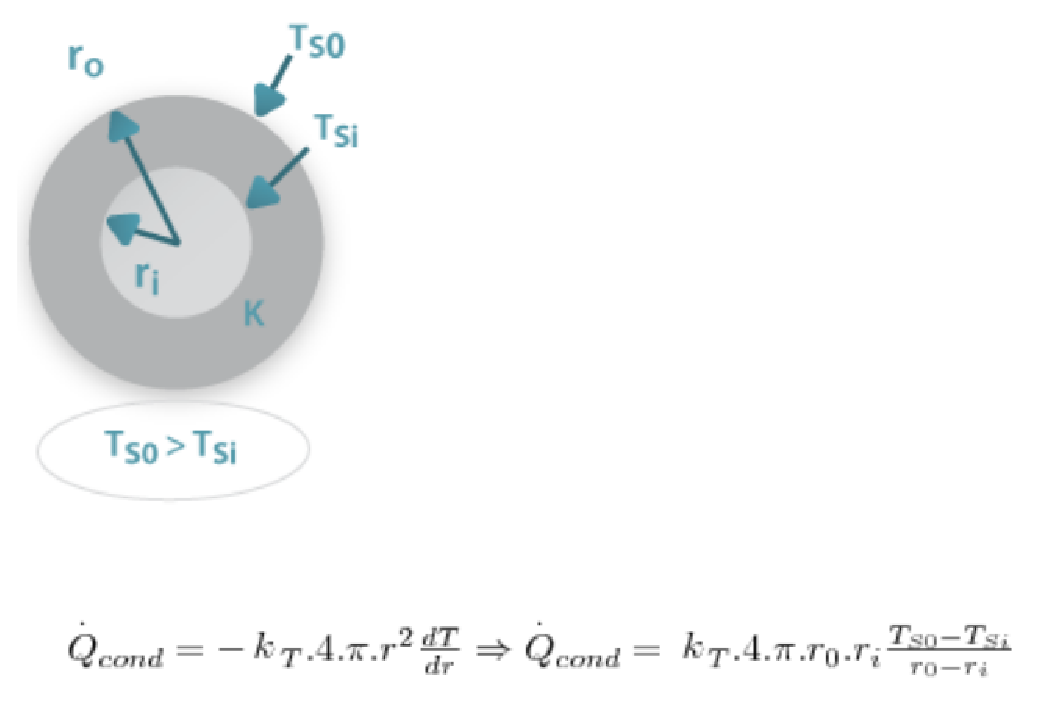
\includegraphics[width=15cm, keepaspectratio=true]{figuras/Teste12.eps}
   \caption{Esquemático geral do projeto de estrutura}                        
\end{figure}

$$ Q_{cond} = k_{t}.4.\pi.r^2.\frac{dT}{dr} \Longrightarrow Q_{cond} = k_{t}.4.\pi.r_{0}.r_{i}.\frac{T_{S0}-T_{Si}}{r_{0}-r_{i}}$$


\subsection{Análise das tubulações}

\subsubsection{Condutividade térmica}
O mecanismo da Condução de calor está associado à transferência de calor efectuada ao nível molecular, por transferência de energia sensível. O calor transferido por unidade de tempo, ou a velocidade de transferência de calor, na direcção x é proporcional à área de transferência perpendicular ao fluxo de calor $A=WxH, m2$, e ao gradiente de temperaturas $\frac{dT}{dx}$.

Para as geometrias cilíndrica e esférica (como no caso de escoamento de fluidos no interior de condutas cuja parede está mais quente ou mais fria), e considerando o fluxo de calor exclusivamente na direção radial, obtém-se a Equação abaixo, onde $K_{t}$ é o coeficiente de transferência térmica ,presente na Tabela 2, L é o comprimento, r o raio e T a temperatura.
$$ Q_{cond} = -k_{t}.2\pi.r.L.\frac{dT}{dr} \Longrightarrow Q_{cond} = k_{t}.2\pi.L.\frac{T_{S0}-T_{Si}}{\ln (r_{0}-r_{i})}$$

O comprimento total do tubo é de 6 m, o diâmetro interno equivale a 4 mm e a espessura a 1mm, e o valor da temperatura interna aproximadamente $50^{\circ}C$ e a temperatura externa com valor em torno de $30^{\circ}C$. A partir disso, concluiu-se que o valor Q equivale a 464,89 W.

\subsubsection{Material}
Para as mangueiras e conectores da condução do líquido de arrefecimento, o material utilizado será o politetrafluoretileno (PTFE), popularmente conhecido como teflon. As principais características desse plástico fluorado é sua inércia química, estabilidade em altas e baixas temperaturas, excelentes propriedades elétricas e baixo coeficiente de atrito.

As resinas de PTFE são opacas, cristalizadas e maleáveis. Quando aquecidas acima de $340^{\circ}C$, tornam-se transparentes, amorfas e de tratamento relativamente difícil, sofrendo fraturas quando severamente deformadas. Ao serem resfriadas, voltam ao seu estado original. Geralmente são utilizadas em aplicações nas quais se aproveitam suas propriedades elétricas, químicas e mecânicas fora do comum, mas também em componentes de sistemas de transportes de fluidos, peças moldadas de ajuste e vedação, entre outros.\\

A alta resistência ao calor e outras características do PTFE, listadas na Tabela 1, foram os principais critérios utilizados para escolha do material.\\



Entretanto, para o adaptador que liga a pós-câmara ao sensor de pressão é empregado o Aço Inoxidável (AISI 304L). A escolha do material foi determinada por meio das propriedades físicas e químicas, entre elas : apresenta boa resistência à corrosão e resistência à oxidação de até $850^{\circ}C$ , permite excelente maquinabilidade, o material é muito dúctil sendo de fácil estampagem e  embutidura.

Assim a tabela 02 demonstra as principais características do AISI 304 L.


\subsubsection{Dimensões}
De acordo com o modelo feito para o posicionamento da bomba, os materiaisnecessários, do sistema até a chegada ao sensor serão:
\begin{itemize}
\item 6m de mangueira (Ø = 4mm)
\item 4 cotovelos
\item 2 adaptadores "Tês"
\end{itemize}

Já para o tubo que conecta ao sensor é necessário um ducto de Ø =19mm por 100mm de comprimento. Dessa forma, conforme a imagem abaixo, a qual refere-se ao corte horizontal do tubo percebe-se um furo com Ø =3mm na maior parte de extensão.


\subsubsection{Simulações}
Após a realização dos cálculos por meio de modelos matemáticos Newtonianos, é necessária a realização de simulações para que possam garantir que as operações foram efetuadas corretamente e assim, diminuir a porcentagem de erros e riscos. O software utilizado foi o ANSYS versão R18.1 Academic.

\begin{figure}[!htb]                                                               
   \centering                                                                      
   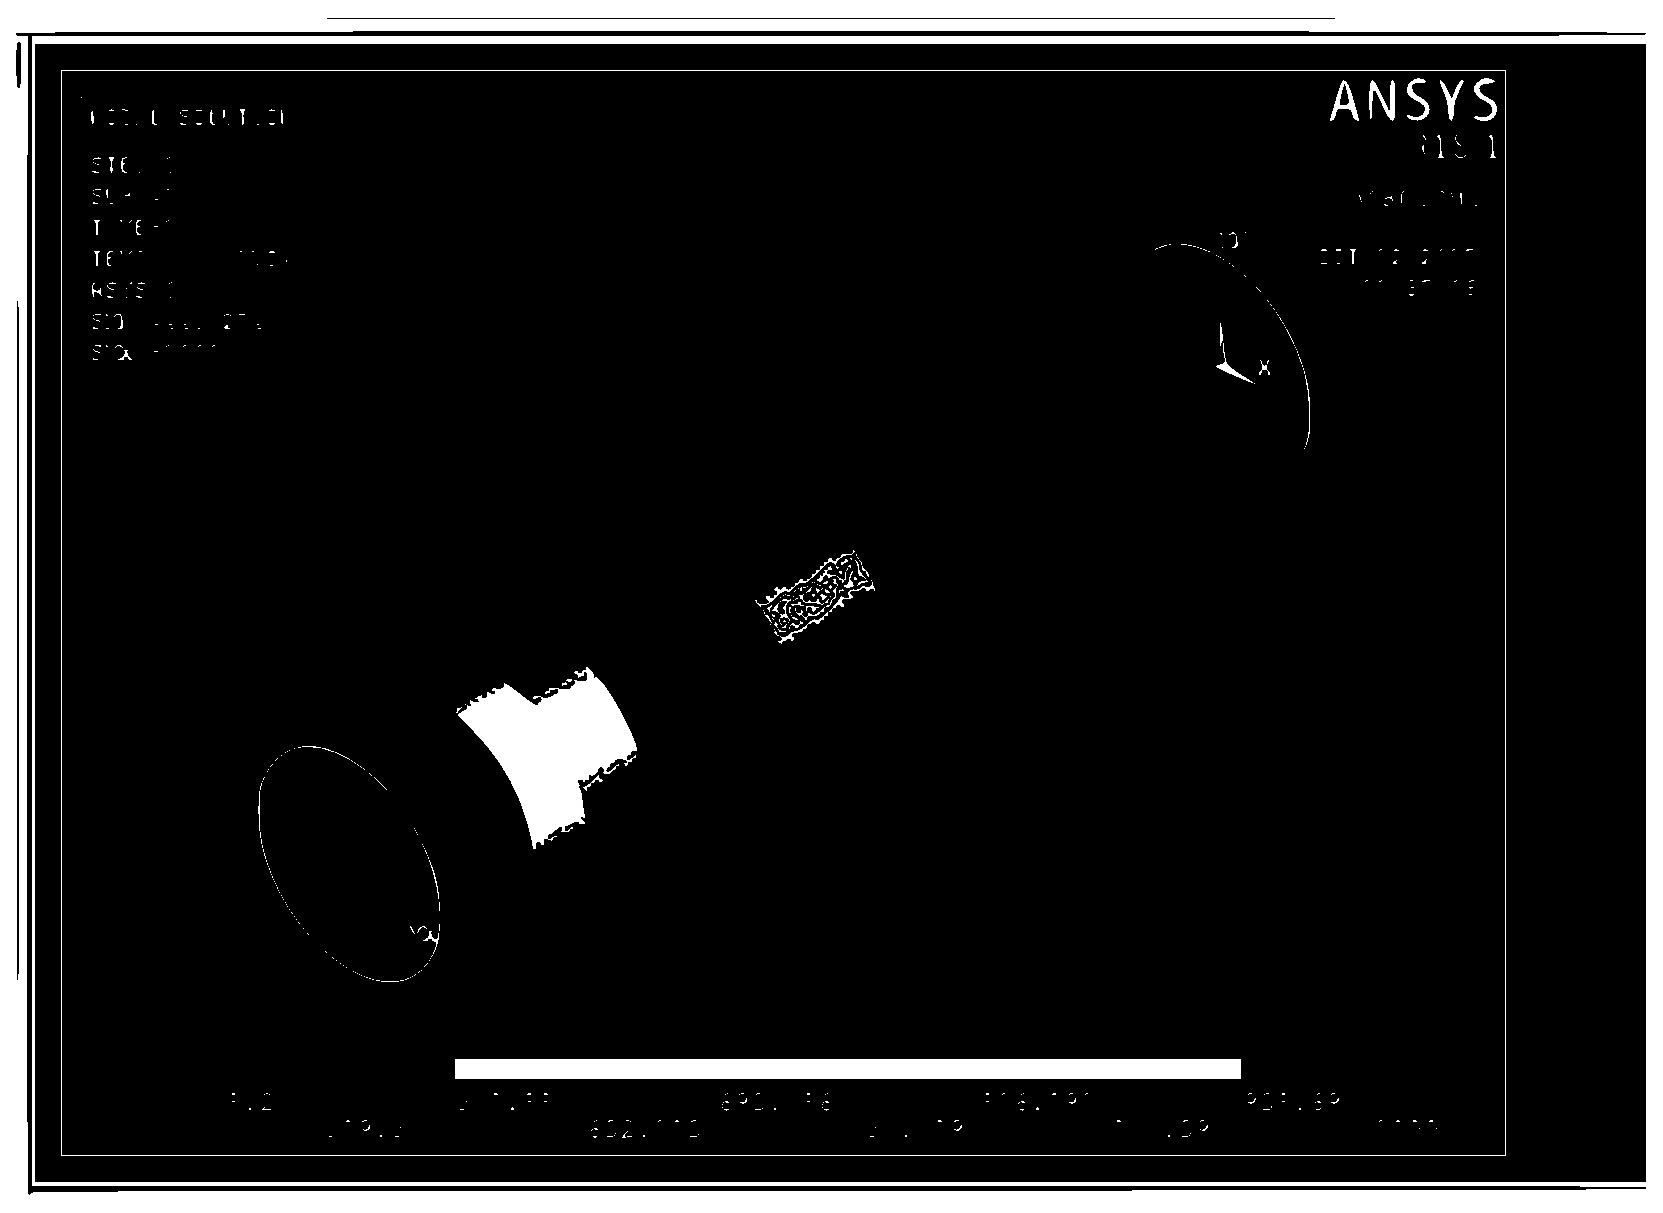
\includegraphics[width=15cm, keepaspectratio=true]{figuras/Resultado1.eps}
   \caption{Esquemático geral do projeto de estrutura}                        
\end{figure}

Consequentemente, para a segunda etapa o software utilizado foi o ANSYS versão R18.2 Academic. Assim, para realizar o estudo termodinâmico do tubo, o qual liga a pós-câmara ao sensor de pressão é empregado o Steady-State Thermal (Estado Térmico Estacionário), entretanto para uma maior precisão é necessária a realização de um estudo em um estado transiente, que depende do menor e maior tempo de excução do motor. Com tal característica, utiliza-se como geometria um cilindro de 19 mm de diâmetro para facilitar a simulação e dessa forma não tem grandes alterações no resultado final.

\subsection{Riscos na transmissão de calor}

Visto que o nosso grupo se dispões apenas de ferramentas teóricas, seus riscos também se mantêm em tal perspectiva de forma que os únicos riscos existentes em tal processo sejam apenas técnicos e administrativos.

\subsubsection{Riscos técnicos}
Nas utilizações das fórmulas e nas simulações podem existir erros contidos tanto na medição das variáveis iniciais, determinando assim uma propagação de erros muito grande levando em consideração o processo inteiro e a utilização de medidas experimentais industriais sem erro definido aumentando assim sua variabilidade, pensando nisso a solução utilizada no projeto e aconselhada pelos professores é tanto a simplificação quanto a utilização de fatores de seguranças mais razoáveis que a média, de forma que o ponto do projeto é o custo benefício assim, todo e qualquer erro pode ser absorvido por um custo de produção baixo.

A utilização de softwares também diminui consideravelmente esse erro visto que sua capacidade para erros é menor de acordo com o grau da simulação, por isso a utilização da maior resolução possível em simulações utilizadas.

As únicas medida de contenção que se restringe à essa parte é a reavaliação dos processos e sua imediata substituição pelos dados revisados.

\subsubsection{Riscos admnistrativos}

Os riscos mais prováveis em nossa desenvolvimento visto que nossa natureza estudantil nos leva a erros administrativos, a utilização de recursos humanos à sua potencialidade foi um dos problemas encontrados pelo grupo e o controle de pessoal, de forma que esses poderiam desestruturar o funcionamento, sendo eles o descumprimento de prazos, falta de pessoal e impossibilidade de reuniões os maiores contribuintes nessa soma.

\subsection {Orçamentos}

\begin{table}[htb]
\begin{tabular}{|p{3cm}|p{4cm}|p{3cm}|}
\hline
Recurso & Descrição & Preço(R\$) \\
\hline
Mão-de-obra & 5 estagiários com 18 horas mensais para cada e considerando um salário base de R\$1000,00 de 120 horas mensais & 150,00 * 5 = 750,00\\ \hline
Software Ansys & Versão estudante com algumas limitações & 0,00\\ \hline
\hline
\end{tabular}
\caption{Orçamentos da divisão Transmissão de calor}
\end{table}

\subsection{Resultados}

Independentemente do sistema de proteção térmica, a previsão do fluxo de calor é uma tarefa de extrema importância, tanto em motores foguete a propelente líquido quanto em motoresa propelente sólido pois se trata de um aspecto que limita a performance do propulsor, forçando muitas vezes o processo de combustão ser ajustado para operar fora do ponto estequiométrico dos propelentes envolvidos para reduzir a temperatura dos gases quentes, evitando extrair a máxima eficiência energética dos propelentes (PATIRE JR, 2010).

O líquido escolhido foi a água pela suas propriedades e pela facilidade encontrada para análises com base em dados disponibilizados pela fabricante, agilizando ,assim como, redução dos cálculos, além da facilidade de obtenção sendo praticamente gratuito e abundante. As presentes afirmações foram consideradas com base em datasheets e contextualização do projeto para materiais de fácil aquisição.

Consequentemente, a determinação dos principais parâmetros para o segundo ponto de controle foram formuladas pelas análises teóricas e depois foram comprovadas pelo uso do simulador Ansys. De modo similar, a escolha dos materiais são concretizadas pelos cálculos, adaptando as propriedades físicas e químicas de cada material aos requisitos térmicos do sistema.

Dessa forma, como previsto anteriormente o projeto em questão é plausível e assim desloca-se para uma resolução certeira.

\subsection{Discussões e Conclusões}

Após todos esses passos, os resultados encontrados nas funções que cabiam ao grupo, após a simulação do cilindro é de $450^{\circ}C$ na ponta do adaptador, a temperatura da água não passa de $60^{\circ}C$ e o sensor sobreviverá à temperatura que se encontra no motor se o sistema de arrefecimento funcionar corretamente, realizando as medições necessárias entre os períodos de tempo do teste, sendo eles entre 15 e 60 segundos.
